\normaltrue
\correctionfalse

%\UPSTIidClasse{11} % 11 sup, 12 spé
%\newcommand{\UPSTIidClasse}{12}

\exer{Mouvement RR  $\star$ \label{C2:08:04}}
\setcounter{question}{0}\UPSTIcompetence[2]{C2-08}
\UPSTIcompetence[2]{C2-09}
\index{Compétence C2-08}
\index{Compétence C2-09}
\index{Torseur cinétique}
\index{Torseur dynamique}
\index{Mécanisme à 2 rotations}
\ifcorrection
\else
\textbf{Pas de corrigé pour cet exercice.}
\fi

\ifprof
\else
Soit le mécanisme suivant. On a $\vect{AB}=R\vect{i_1}$ avec $R=\SI{20}{mm}$ et  
$\vect{BC}=L\vect{i_2}$ avec $L=\SI{15}{mm}$. De plus :
\begin{itemize}
\item $G_1$ désigne le centre d'inertie de \textbf{1} et $\vect{AG_1}=\dfrac{1}{2}R\vect{i_1}$, on note $m_1$ la masse de \textbf{1} et $\inertie{G_1}{1}=\matinertie{A_1}{B_1}{C_1}{0}{0}{0}{\bas{1}}$; 
\item $G_2$ désigne le centre d'inertie de \textbf{2} et $\vect{BG_2}=\dfrac{1}{2}L\vect{i_2}$, on note $m_2$ la masse de \textbf{2} et $\inertie{G_2}{2}=\matinertie{A_2}{B_2}{C_2}{0}{0}{0}{\bas{2}}$.
\end{itemize}
\begin{center}
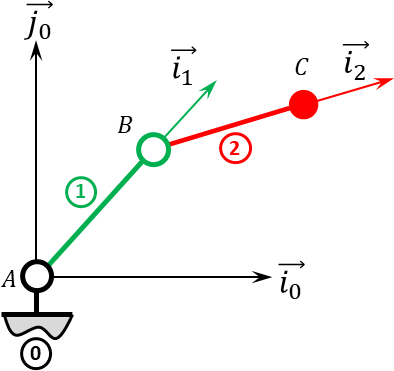
\includegraphics[width=\linewidth]{04_RR_01}
\end{center}
\fi

\question{Exprimer le torseur dynamique $\torseurdyn{1}{0}$ en $A$ en utilisant 2 méthodes différentes pour le calcul du moment.}
\ifprof

[NON TERMINE]
\textbf{Définition}

$\torseurdyn{1}{0} = \torseurl{m_1 \vectg{G_1}{1}{0}}{\babard{A}{G_1}{1}{0}}{A}$

\textbf{Calcul de $\vectv{G_1}{1}{0}$}

$\vectv{G_1}{1}{0}$ $ = \deriv{\vect{AG_1}}{\rep{0}}$
$ = \dfrac{1}{2}R\deriv{\vect{i_1}}{\rep{0}}$
$ = R\dot{\theta}\vj{1}$.

(Avec $\deriv{\vect{i_1}}{\rep{0}} = \deriv{\vect{i_1}}{\rep{1}} + \vecto{1}{0}\wedge \vi{1}$
$ = \dot{\theta}\vk{0}\wedge \vi{1}$ $ = \dot{\theta}\vj{1}$).

\textbf{Calcul de $\vectg{G_1}{1}{0}$}

$\vectg{G_1}{1}{0}$ $ = \deriv{{\vectv{G_1}{1}{0}}}{\rep{0}}$
$ =  R\ddot{\theta}\vj{1} - R\dot{\theta}^2\vi{1} $.

\textbf{Calcul de $\vectmc{G_1}{1}{0}$}

$G_1$ est le centre d'inertie de 1; donc : 
$\vectmc{G_1}{1}{0} = \inertie{G_1}{1}\vecto{1}{0} = \thetap C_1 \vz{1}$.

\textbf{Calcul de $\vectmd{G_1}{1}{0}$}

$G_1$ est le centre d'inertie de 1; donc : 
$\vectmd{G_1}{1}{0} = \deriv{\vectmc{G_1}{1}{0}}{\rep{0}} = \thetapp C_1 \vz{1}$.

\textbf{Calcul de $\vectmd{A}{1}{0}$}

En utilisant la formule de changement de point, on a : 
$\babard{A}{G_1}{1}{0} = \thetapp C_1 \vz{1} + \dfrac{1}{2}R\vi{1} \wedge m_1 \left( R\ddot{\theta}\vj{1} - R\dot{\theta}^2\vi{1}\right)$

\else
\fi

\question{Exprimer le torseur dynamique $\torseurdyn{2}{0}$ en $B$ en utilisant 2 méthodes différentes pour le calcul du moment.}
\ifprof

$\vectv{C}{2}{0}$ $ = \deriv{\vect{AC}}{\rep{0}}$
$ = \deriv{\vect{AB}}{\rep{0}}+\deriv{\vect{BC}}{\rep{0}}$
$ = R\deriv{\vect{i_1}}{\rep{0}}+L\deriv{\vect{i_2}}{\rep{0}}$
$ = R\dot{\theta}\vj{1}+L\left( \dot{\theta}+\dot{\varphi}\right)\vj{2}$.

(Avec $\deriv{\vect{i_2}}{\rep{0}} = \deriv{\vect{i_2}}{\rep{2}} + \vecto{2}{0}\wedge \vi{2}$
$ = \left( \dot{\theta}+\dot{\varphi}\right)\vk{0}\wedge \vi{2}$ $ = \left( \dot{\theta}+\dot{\varphi}\right)\vj{2}$).

\else
\fi

\question{Déterminer $\vectmd{A}{1+2}{0}\cdot \vect{k_0}$.}
\ifprof
\else
\fi

\ifcolle
\question{Déterminer $\pext{2}{1}{0}$ et $\pext{1}{2}{0}$.}
\else
\fi


\ifprof
\else
\begin{flushright}
\footnotesize{Corrigé  voir \ref{C2:08:04}.}
\end{flushright}%
\fi